\subsection{Adding-Like}

Scenario like the original model.

\begin{figure}
    \centering
    \begin{subfigure}{0.4\textwidth}
        \centering
        \includegraphics[width=\textwidth]{70_030_SearchAdding_quad2/2D_Period_LowerLeft/result.png}
        \caption{Periods}
        %        \label{fig:final.period.whole.full}
    \end{subfigure}
    \begin{subfigure}{0.4\textwidth}
        \centering
        \includegraphics[width=\textwidth]{70_030_SearchAdding_quad2/2D_Regions_LowerLeft/result.png}
        \caption{Period Regions}
        %        \label{fig:final.period.whole.halved}
    \end{subfigure}
    \caption{2D Scans of Periods and Period Regions of Lower Left Quarter Of Quad2 Model}
\end{figure}

\begin{figure}
    \centering
    \begin{subfigure}{0.3\textwidth}
        \centering
        \includegraphics[width=\textwidth]{70_030_SearchAdding_quad2/Cobweb_LowerLeft_A13/result.png}
        \caption{At $A_{13}$}
        %        \label{fig:final.period.whole.full}
    \end{subfigure}
    \begin{subfigure}{0.3\textwidth}
        \centering
        \includegraphics[width=\textwidth]{70_030_SearchAdding_quad2/Cobweb_LowerLeft_B13/result.png}
        \caption{At $B_{13}$}
        %        \label{fig:final.period.whole.halved}
    \end{subfigure}
    \begin{subfigure}{0.3\textwidth}
        \centering
        \includegraphics[width=\textwidth]{70_030_SearchAdding_quad2/Cobweb_LowerLeft_C13/result.png}
        \caption{At $C_{13}$}
        %        \label{fig:final.period.whole.halved}
    \end{subfigure}
    \caption{Cobwebs at Selected Points of Lower Left Quarter Of Quad2 Model}
\end{figure}
